\documentclass[12pt,a4paper]{article}

% ─── Page Layout ───────────────────────────────────────────────────────────────
\usepackage[a4paper, margin=0.8in, headheight=14pt]{geometry}

% ─── Fonts (XeLaTeX) ───────────────────────────────────────────────────────────
\usepackage{fontspec}
\usepackage{unicode-math}
\setmainfont{TeX Gyre Pagella}
\setmonofont[Scale=0.88]{TeX Gyre Cursor}
\setmathfont{Latin Modern Math}

% ─── Packages ──────────────────────────────────────────────────────────────────
\usepackage{xcolor}
\usepackage{colortbl}
\usepackage{titlesec}
\usepackage{enumitem}
\usepackage{tabularx}
\usepackage{booktabs}
\usepackage{array}
\usepackage{amsmath}
\usepackage{tikz}
\usetikzlibrary{shapes.geometric, arrows.meta, positioning, calc, fit, decorations.pathreplacing}
\usepackage{tcolorbox}
\tcbuselibrary{skins, breakable}
\usepackage{hyperref}
\usepackage{fancyhdr}
\usepackage{graphicx}
\usepackage{microtype}
\hyphenpenalty=10000
\exhyphenpenalty=10000
\sloppy
\usepackage{caption}
\usepackage{setspace}
\usepackage{multirow}
\usepackage{tocloft}

% ─── Q&A helper ────────────────────────────────────────────────────────────────
\newcommand{\Q}[1]{\textbf{#1}\par\noindent\ignorespaces}

% ─── Colour Palette ────────────────────────────────────────────────────────────
\definecolor{myred}{RGB}{196,30,58}
\definecolor{mydark}{RGB}{30,30,50}
\definecolor{mygreen}{RGB}{14,120,80}
\definecolor{myteal}{RGB}{0,130,140}
\definecolor{myamber}{RGB}{180,100,0}
\definecolor{mypurple}{RGB}{100,30,160}
\definecolor{mygray}{RGB}{246,247,249}
\definecolor{mgframe}{RGB}{180,185,200}
\definecolor{watermark}{RGB}{145,150,170}
\definecolor{hdrred}{RGB}{250,232,235}
\definecolor{hdrgreen}{RGB}{220,244,233}
\definecolor{hdrteal}{RGB}{220,242,244}
\definecolor{hdramber}{RGB}{253,242,215}
\definecolor{hdrpurple}{RGB}{238,228,255}
\definecolor{hdrgray}{RGB}{238,240,245}
\definecolor{rowalt}{RGB}{250,251,253}

% ─── Section Formatting ────────────────────────────────────────────────────────
\titleformat{\section}
  {\large\bfseries\color{myred}}{\thesection.}{0.5em}{}
  [\vspace{1pt}{\color{myred}\rule{\linewidth}{0.8pt}}]
\titleformat{\subsection}
  {\normalsize\bfseries\color{myteal}}{\thesubsection}{0.5em}{}
\titlespacing*{\section}{0pt}{18pt}{7pt}
\titlespacing*{\subsection}{0pt}{11pt}{4pt}

% ─── Paragraph ─────────────────────────────────────────────────────────────────
\setlength{\parindent}{0pt}
\setlength{\parskip}{4pt}

% ─── TOC Styling ───────────────────────────────────────────────────────────────
\renewcommand{\cfttoctitlefont}{\large\bfseries\color{myred}}
\renewcommand{\cftaftertoctitle}{\par\noindent{\color{myred}\rule{\linewidth}{0.8pt}}}
\setlength{\cftbeforetoctitleskip}{0pt}
\setlength{\cftaftertoctitleskip}{6pt}
\renewcommand{\cftsecfont}{\normalsize\bfseries\color{mydark}}
\renewcommand{\cftsecpagefont}{\normalsize\bfseries\color{mydark}}
\renewcommand{\cftsecleader}{\cftdotfill{\cftdotsep}}
\setlength{\cftbeforesecskip}{7pt}
\renewcommand{\cftsubsecfont}{\small\color{mydark}}
\renewcommand{\cftsubsecpagefont}{\small\color{mydark}}
\setlength{\cftbeforesubsecskip}{3pt}
\setlength{\cftsubsecindent}{1.4em}

% ─── Table helpers ─────────────────────────────────────────────────────────────
\renewcommand{\arraystretch}{1.45}
\setlength{\tabcolsep}{6pt}
\arrayrulecolor{mydark}
\newcolumntype{B}[1]{>{\small\bfseries\raggedright\arraybackslash}m{#1}}
\newcolumntype{Y}{>{\small\raggedright\arraybackslash}X}
\renewcommand{\tabularxcolumn}[1]{m{#1}}

% ─── Header / Footer ───────────────────────────────────────────────────────────
\pagestyle{fancy}
\fancyhf{}
\fancyhead[L]{\small\color{myred}\textbf{OE-EC604C}\;\color{mydark}--- Object Oriented Programming}
\fancyhead[R]{\small\color{myteal}\textbf{Module 4 Notes}}
\fancyfoot[C]{\small\color{mydark}\thepage}
\fancyfoot[R]{\small\color{watermark}\textit{\copyright\ Biraj}}
\renewcommand{\headrulewidth}{0.5pt}
\renewcommand{\footrulewidth}{0.3pt}

% ─── Hyperref ──────────────────────────────────────────────────────────────────
\hypersetup{
  colorlinks=true, linkcolor=myteal, urlcolor=myteal,
  pdfauthor={Biraj Sarkar},
  pdftitle={OE-EC604C --- Module 4 Notes}
}

% ─── tcolorbox styles ──────────────────────────────────────────────────────────
\tcbset{
  tikzbox/.style={
    colback=mygray, colframe=mgframe, boxrule=0.6pt, arc=4pt,
    left=8pt, right=8pt, top=6pt, bottom=6pt,
    colbacktitle=mgframe, coltitle=mydark,
    fonttitle=\small\bfseries
  },
  defbox/.style={
    colback=hdrgreen, colframe=mygreen, boxrule=0.8pt, arc=4pt,
    left=9pt, right=9pt, top=6pt, bottom=6pt,
    colbacktitle=mygreen, coltitle=white,
    fonttitle=\small\bfseries
  },
  formulabox/.style={
    colback=hdrteal, colframe=myteal, boxrule=0.8pt, arc=4pt,
    left=9pt, right=9pt, top=7pt, bottom=7pt,
    colbacktitle=myteal, coltitle=white,
    fonttitle=\small\bfseries
  },
  examplebox/.style={
    colback=hdramber, colframe=myamber, boxrule=0.8pt, arc=4pt,
    left=9pt, right=9pt, top=6pt, bottom=6pt,
    colbacktitle=myamber, coltitle=white,
    fonttitle=\small\bfseries
  },
  masonbox/.style={
    colback=hdrpurple, colframe=mypurple, boxrule=0.8pt, arc=4pt,
    left=9pt, right=9pt, top=6pt, bottom=6pt,
    colbacktitle=mypurple, coltitle=white,
    fonttitle=\small\bfseries
  },
  exambox/.style={
    colback=hdrpurple, colframe=mypurple, boxrule=1pt, arc=5pt,
    left=10pt, right=10pt, top=8pt, bottom=8pt,
    colbacktitle=mypurple, coltitle=white,
    fonttitle=\bfseries,
    breakable, title after break={\textbf{Frequently Asked / Viva Questions (contd.)}}}
}

% XeLaTeX pdfcol fix: reset text color after every tcolorbox
\tcbset{after={\color{black}}}

% ─── TikZ styles ───────────────────────────────────────────────────────────────
\tikzset{
  block/.style={rectangle, draw=myteal, fill=hdrteal,
    text width=2.4cm, align=center, minimum height=0.95cm,
    font=\small, rounded corners=3pt, line width=0.7pt},
  redblock/.style={rectangle, draw=myred, fill=hdrred,
    text width=2.4cm, align=center, minimum height=0.95cm,
    font=\small, rounded corners=3pt, line width=0.7pt},
  netnode/.style={rectangle, draw=myteal, fill=hdrteal,
    text width=1.5cm, align=center, minimum height=0.8cm,
    font=\small, rounded corners=3pt, line width=0.7pt},
  sumjunc/.style={circle, draw=myamber, fill=hdramber,
    minimum size=0.62cm, font=\small, line width=0.8pt},
  snode/.style={circle, draw=mypurple, fill=hdrpurple,
    minimum size=0.55cm, font=\footnotesize, line width=0.7pt},
  arrow/.style={-Stealth, thick, color=mydark},
  redarrow/.style={-Stealth, thick, color=myred},
  line/.style={thick, color=mydark}
}

% ═══════════════════════════════════════════════════════════════════════════════
\begin{document}
% ═══════════════════════════════════════════════════════════════════════════════

\begin{center}
  {\LARGE\bfseries\color{myred} OE-EC604C --- Object Oriented Programming}\\[5pt]
  {\normalsize\color{mydark} Semester VI \quad$\bullet$\quad 3L:0T:0P \quad$\bullet$\quad 3 Credits}\\[3pt]
  {\normalsize\color{myteal}\textbf{Module 4 Exam Notes: Constructors and Destructors}}\\[3pt]
  {\small\color{mydark} CGEC \;$|$\; B.Tech ECE (2023--27) \;$|$\; \textit{Biraj Sarkar}}
\end{center}
\vspace{2pt}
\noindent{\color{myred}\rule{\linewidth}{1.5pt}}
\vspace{2pt}

\hypersetup{linkcolor=mydark}
\tableofcontents
\hypersetup{linkcolor=myteal}
\newpage

% ===============================================================================
\section{Fundamentals of Constructors}
% ===============================================================================

Constructors are special member functions of a class designed specifically to initialize objects during instantiation.

\subsection{Rules and Characteristics}
A constructor must follow strict compiler rules:
\begin{itemize}[leftmargin=*, itemsep=3pt]
  \item \textbf{Naming:} It must have the exact same name as the class.
  \item \textbf{Return Type:} It does not have any return type, not even \texttt{void}.
  \item \textbf{Execution:} It is automatically invoked by the system when an object of the class is created.
  \item \textbf{Implicit/Explicit Invocation:} 
    \begin{align}
      &\text{Implicit call: } \texttt{Complex c1(5, 10);} \\
      &\text{Explicit call: } \texttt{Complex c1 = Complex(5, 10);}
    \end{align}
  \item \textbf{Restrictions:} It cannot be declared \texttt{virtual}, \texttt{static}, or \texttt{const}.
\end{itemize}

\subsection{Types of Constructors}
\begin{enumerate}[label=\textbf{\arabic*.}, leftmargin=*, itemsep=4pt]
  \item \textbf{Default Constructor:} A constructor that accepts no arguments. If no constructor is written, the compiler automatically generates a default constructor.
  \item \textbf{Parameterized Constructor:} A constructor that accepts arguments, allowing objects to be initialized with custom values at creation time.
  \item \textbf{Copy Constructor:} Used to initialize an object using values of another pre-existing object of the same class.
  \item \textbf{Dynamic Constructor:} A constructor that uses the \texttt{new} operator to allocate dynamic heap memory for members during object creation.
\end{enumerate}

% ===============================================================================
\section{Deep Copying and Shallow Copying}
% ===============================================================================

Copy operations in C++ can lead to critical memory bugs if pointers are involved.

\subsection{Shallow Copy vs. Deep Copy}
\begin{itemize}[leftmargin=*, itemsep=3pt]
  \item \textbf{Shallow Copy:} The compiler copies member variables bit-by-bit. If a class contains pointers to heap memory, only the address is copied. As a result, both the original and copied objects point to the same memory block.
    \begin{tcolorbox}[defbox]
    \textbf{Shallow Copy Risk:} When either object is destroyed, its destructor runs and frees the shared heap memory. The remaining object is left with a dangling pointer, and attempting to delete it results in a double-free crash.
    \end{tcolorbox}
  \item \textbf{Deep Copy:} A user-defined copy constructor allocates a separate block of heap memory and copies the actual values from the source buffer. This isolates the memory blocks.
\end{itemize}

\begin{tcolorbox}[tikzbox, title={Memory Block Mappings: Shallow Copy vs. Deep Copy}]
\centering
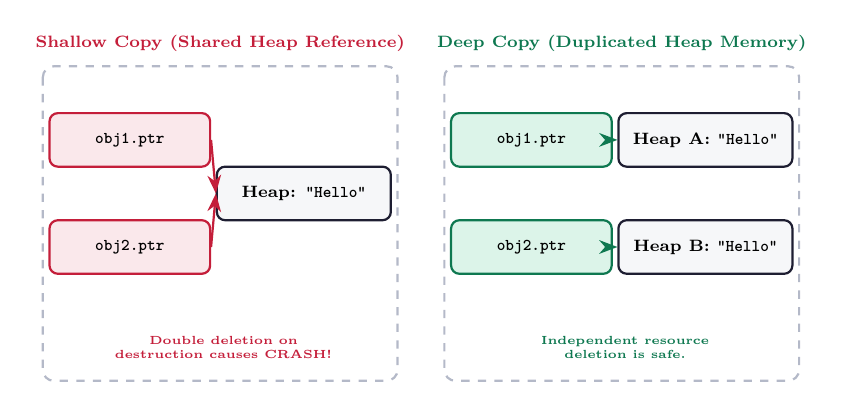
\begin{tikzpicture}[node distance=1.2cm, thick, scale=0.85, every node/.style={scale=0.85}]
  % --- SHALLOW COPY BLOCK ---
  \draw[dashed, color=mgframe, line width=0.8pt, rounded corners=4pt] (-4.5, 2.1) rectangle (0.8, -2.6);
  \node[above=2pt, font=\scriptsize\bfseries\color{myred}] at (-1.85, 2.1) {Shallow Copy (Shared Heap Reference)};
  
  \node[draw=myred, fill=hdrred, rounded corners=3pt, minimum width=2.4cm, minimum height=0.8cm, font=\scriptsize\bfseries] (s_obj1) at (-3.2, 1.0) {\texttt{obj1.ptr}};
  \node[draw=myred, fill=hdrred, rounded corners=3pt, minimum width=2.4cm, minimum height=0.8cm, font=\scriptsize\bfseries] (s_obj2) at (-3.2, -0.6) {\texttt{obj2.ptr}};
  
  \node[draw=mydark, fill=mygray, rounded corners=3pt, minimum width=2.6cm, minimum height=0.8cm, font=\scriptsize\bfseries] (s_heap) at (-0.6, 0.2) {Heap: \texttt{"Hello"}};
  
  \draw[redarrow] (s_obj1.east) -- (s_heap.west);
  \draw[redarrow] (s_obj2.east) -- (s_heap.west);
  \node[below, font=\tiny\bfseries\color{myred}, align=center] at (-1.8, -1.8) {Double deletion on\\destruction causes CRASH!};

  % --- DEEP COPY BLOCK ---
  \draw[dashed, color=mgframe, line width=0.8pt, rounded corners=4pt] (1.5, 2.1) rectangle (6.8, -2.6);
  \node[above=2pt, font=\scriptsize\bfseries\color{mygreen}] at (4.15, 2.1) {Deep Copy (Duplicated Heap Memory)};
  
  \node[draw=mygreen, fill=hdrgreen, rounded corners=3pt, minimum width=2.4cm, minimum height=0.8cm, font=\scriptsize\bfseries] (d_obj1) at (2.8, 1.0) {\texttt{obj1.ptr}};
  \node[draw=mygreen, fill=hdrgreen, rounded corners=3pt, minimum width=2.4cm, minimum height=0.8cm, font=\scriptsize\bfseries] (d_obj2) at (2.8, -0.6) {\texttt{obj2.ptr}};
  
  \node[draw=mydark, fill=mygray, rounded corners=3pt, minimum width=2.6cm, minimum height=0.8cm, font=\scriptsize\bfseries] (d_heap1) at (5.4, 1.0) {Heap A: \texttt{"Hello"}};
  \node[draw=mydark, fill=mygray, rounded corners=3pt, minimum width=2.6cm, minimum height=0.8cm, font=\scriptsize\bfseries] (d_heap2) at (5.4, -0.6) {Heap B: \texttt{"Hello"}};
  
  \draw[arrow, color=mygreen] (d_obj1.east) -- (d_heap1.west);
  \draw[arrow, color=mygreen] (d_obj2.east) -- (d_heap2.west);
  \node[below, font=\tiny\bfseries\color{mygreen}, align=center] at (4.2, -1.8) {Independent resource\\deletion is safe.};
\end{tikzpicture}
\end{tcolorbox}

\begin{tcolorbox}[examplebox, title={Code Example: String copy constructor (Deep Copy)}]
\begin{spacing}{1.0}
\begin{verbatim}
#include <iostream>
#include <cstring>
class String {
private:
    char *str;
    int len;
public:
    String(const char *s) {
        len = strlen(s);
        str = new char[len + 1];
        strcpy(str, s);
    }
    // Deep Copy Constructor
    String(const String &source) {
        len = source.len;
        str = new char[len + 1]; // Allocate separate heap memory
        strcpy(str, source.str); // Copy actual data contents
        std::cout << "Copy Constructor Called (Deep Copy)" << std::endl;
    }
    ~String() {
        delete[] str; // Free local pointer safely
    }
    void display() { std::cout << str << std::endl; }
};
\end{verbatim}
\end{spacing}
\end{tcolorbox}

% ===============================================================================
\section{Constructor Overloading \& Destructors}
% ===============================================================================

C++ allows multiple constructors in a class, selecting the correct one based on arguments. It also ensures proper cleanup when objects go out of scope.

\subsection{Constructor Overloading and Default Arguments}
Classes can have multiple constructors with different parameter signatures. They can also contain default arguments.
\begin{align*}
  &\text{Constructor 1 (Default): } && \texttt{Complex() \{ real = imag = 0; \}} \\
  &\text{Constructor 2 (Parameterized): } && \texttt{Complex(double r, double i = 0) \{ real = r; imag = i; \}}
\end{align*}

\subsection{Destructors}
\begin{tcolorbox}[defbox]
\textbf{Destructor:} A special member function of a class that is called automatically when an object goes out of scope or is explicitly deleted. Its purpose is to release resource allocations (like heap memory, open file handlers, socket connections).
\end{tcolorbox}

\textbf{Key Destructor Rules:}
\begin{itemize}[leftmargin=*, itemsep=2pt]
  \item Naming: Same name as class, prefixed with a tilde symbol (\texttt{\textasciitilde}).
  \item Arguments: Cannot take any parameters or return values. Overloading is not possible.
  \item Execution Order: Objects are destroyed in the \textbf{reverse order} of their creation (Last In, First Out).
\end{itemize}

\begin{tcolorbox}[examplebox, title={Code Example: Tracing Constructor and Destructor Executions}]
\begin{spacing}{1.0}
\begin{verbatim}
#include <iostream>
class Trace {
private:
    int id;
public:
    Trace(int val) : id(val) {
        std::cout << "Constructor called for " << id << std::endl;
    }
    ~Trace() {
        std::cout << "Destructor called for " << id << std::endl;
    }
};

void runLocal() {
    std::cout << "--- Enter local scope ---" << std::endl;
    Trace localObj(2);
    std::cout << "--- Exit local scope ---" << std::endl;
}

int main() {
    std::cout << "--- Main Start ---" << std::endl;
    Trace globalObj(1);
    runLocal();
    std::cout << "--- Main End ---" << std::endl;
    return 0;
}
\end{verbatim}
\end{spacing}
\end{tcolorbox}
The code above outputs:
\begin{verbatim}
--- Main Start ---
Constructor called for 1
--- Enter local scope ---
Constructor called for 2
--- Exit local scope ---
Destructor called for 2
--- Main End ---
Destructor called for 1
\end{verbatim}

% ===============================================================================
% MANDATORY QUICK REVISION PAGE
% ===============================================================================
\newpage
\begin{center}
  {\large\bfseries\color{myred} Quick Revision --- Module IV}\\[3pt]
  {\small\color{mydark} Constructors and Destructors $|$ OE-EC604C}
\end{center}
\noindent{\color{myred}\rule{\linewidth}{1.2pt}}
\vspace{4pt}

\begin{tcolorbox}[formulabox, title={\textbf{Key Constructor Syntax}}]
\renewcommand{\arraystretch}{1.3}
\begin{tabularx}{\linewidth}{B{3.8cm} X}
Default Constructor      & \texttt{MyClass() \{ x = 0; \}} \\[4pt]
Parameterized            & \texttt{MyClass(int val) : x(val) \{ \} // uses initializer list} \\[4pt]
Copy Constructor         & \texttt{MyClass(const MyClass \&src) \{ x = src.x; \} // reference is mandatory} \\[4pt]
Destructor               & \texttt{\textasciitilde MyClass() \{ /* release heap memory / close files */ \}}
\end{tabularx}
\end{tcolorbox}

\begin{tcolorbox}[defbox, title={\textbf{One-Line Definitions}}]
\begin{itemize}[leftmargin=*, itemsep=2.5pt, topsep=0pt]
  \item \textbf{Constructor:} A special member function with the class name that initializes objects upon instantiation.
  \item \textbf{Default Constructor:} A constructor that takes no parameters (either empty or with all arguments defaulted).
  \item \textbf{Copy Constructor:} A constructor used to create an object as a clone of an existing object of the same class.
  \item \textbf{Dynamic Constructor:} A constructor that allocates heap memory dynamically during object initialization.
  \item \textbf{Destructor:} A special member function prefixed with \texttt{\textasciitilde} that deallocates resources when an object is destroyed.
  \item \textbf{Shallow Copy:} A member-by-member copy of an object, copying pointer addresses rather than the target data.
  \item \textbf{Deep Copy:} A copy operation that duplicates the heap resources pointed to by an object, creating an independent clone.
  \item \textbf{Initializer List:} A comma-separated list prefixing a constructor body used to initialize data members directly.
  \item \textbf{Double Deletion:} A crash state occurring when two objects point to the same heap block and both attempt to delete it.
\end{itemize}
\end{tcolorbox}

\begin{tcolorbox}[exambox, title={\textbf{Frequently Asked / Viva Questions}}]
\begin{enumerate}[topsep=0pt, label=\textbf{Q\arabic*.}, itemsep=5pt]
  \item \Q{Why is it mandatory to pass the argument by reference in a copy constructor?}
    If passed by value, the function call itself would invoke the copy constructor to clone the parameter, causing infinite recursion until the stack overflows. E.g., \texttt{MyClass(MyClass source)} is incorrect.
  \item \Q{Can a class have more than one destructor?}
    No. Destructors cannot accept arguments, which means they cannot be overloaded. Every class has exactly one destructor.
  \item \Q{Under what conditions does the C++ compiler write a default copy constructor for you?}
    If a class does not define any copy constructor, the compiler automatically generates a default copy constructor, which performs a shallow copy.
  \item \Q{Explain the order of execution of constructors and destructors in hybrid structures.}
    Constructors are invoked in the order of inheritance (base classes first, then derived classes). Destructors run in the exact reverse order.
  \item \Q{Is it possible to declare a private constructor in C++?}
    Yes. A private constructor prevents objects from being created outside the class scope. This pattern is commonly used in the Singleton Design Pattern.
  \item \Q{What is the difference between copy constructor and assignment operator (\texttt{=})?}
    The copy constructor initializes a newly created object using a source object (e.g., \texttt{MyClass a = b;}). The assignment operator copies values to an already existing object (e.g., \texttt{a = b;}).
  \item \Q{Does a destructor release the memory of the object itself?}
    No. A destructor only frees auxiliary resources allocated \textit{inside} the object (e.g., heap pointers, file descriptors). The memory for the object structure itself is freed by the stack or heap manager.
  \item \Q{Why can't we declare a constructor as \texttt{virtual}?}
    Virtual functions rely on the V-Table (virtual table) pointer inside an object. During construction, the object is not fully formed, and the V-Ptr is not yet initialized. Thus, constructors cannot be virtual.
  \item \Q{What is the purpose of declaring copy constructor arguments as \texttt{const}?}
    Declaring the argument as \texttt{const} (e.g., \texttt{const MyClass \&obj}) prevents the copy constructor from accidentally modifying the source object.
  \item \Q{What is a member initializer list and when is it mandatory?}
    It is a constructor mechanism used to initialize members directly. It is mandatory for: (1) initializing reference variables, (2) initializing \texttt{const} members, and (3) calling parameterized base class constructors.
  \item \Q{Can we call a constructor explicitly like a normal function?}
    Yes, we can call it explicitly (e.g., \texttt{Complex c = Complex(1.0, 2.0);}), which creates a temporary object that is then copied or moved.
  \item \Q{What happens if an exception is thrown inside a constructor?}
    If an exception is thrown in a constructor, the object is considered only partially constructed, and its destructor will not run. This can lead to memory leaks unless resources are managed via smart pointers.
\end{enumerate}
\end{tcolorbox}

\begin{tcolorbox}[tikzbox, title={Comparison: Shallow Copy vs. Deep Copy}]
\renewcommand{\arraystretch}{1.45}
\par\noindent
\begin{tabularx}{\linewidth}{|B{3.2cm}|Y|Y|}
\hline
\textbf{Feature} & \textbf{\color{myred}Shallow Copy} & \textbf{\color{mygreen}Deep Copy} \\
\hline
\textbf{Heap Memory} & Shares the existing heap memory between objects. & Allocates new, independent memory blocks on the heap. \\
\hline
\textbf{Pointer Safety} & Pointer address is copied. Vulnerable to dangling pointers. & Pointers point to separate blocks. Safe from cross-corruption. \\
\hline
\textbf{Crash Risk} & High. Double deletion in destructors crashes the program. & Safe. Destructors free distinct blocks independently. \\
\hline
\textbf{Default Behavior} & Executed by default compiler copy constructors. & Must be manually coded by overriding the copy constructor. \\
\hline
\textbf{Execution Speed} & Extremely fast (simple bitwise copy). & Slightly slower (calls heap allocator and copies bytes). \\
\hline
\end{tabularx}
\end{tcolorbox}

\end{document}
